\subsection{Properties of the LCA}
\label{sec:meta}

When merging two concurrent versions $v_1$ and $v_2$, the common
ancestor argument for \C{merge} must be the LCA of $v_1$ and $v_2$,
without which \C{merge} may yield unexpected results. This is
demonstrated for the grow-only counter in
Fig.~\ref{fig:merge-needs-lca}, where an incorrect count is obtained if a
common ancestor that is not an LCA is used to merge 4 and 7. While in
this example there is a unique LCA for 4 and 7, in general this may
\begin{wrapfigure}{l}{.4\textwidth}
\centering
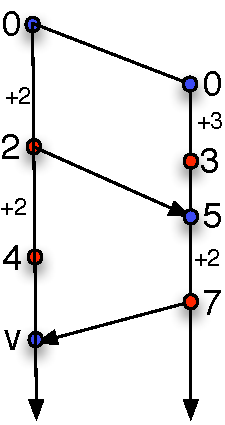
\includegraphics[scale=0.6]{Figures/merge-needs-lca}
\caption{This example of a grow-only counter illustrate why \C{merge}
needs a lowest common ancestor, and not just a common ancestor. Both 0
and 2 are common ancestors of 4 and 7, while 2 is their lowest common
ancestor (since $0 \preceq 2$). The result (v) of merging 4 and 7 is
11 (incorrect) if 0 is used as the common ancestor for merge, and 9
(correct, because 2+2+3+2 = 9) if 2 is used. }
\label{fig:merge-needs-lca}
\end{wrapfigure}
not be the case. With unrestrained branching and merging, there is no
bound on the number of LCAs a pair of versions can have.  For example,
in Fig.~\ref{fig:criss-cross-lcas}, the merge of 0 with 3 is preceded
by two ``criss-cross'' merges between their respective
branches\footnote{
  When discussing merges and LCAs, we often attribute the properties
  of latest versions on branches to the branches themselves.  For
  instance, when we say two branches merge, in fact their latest
  versions merge. Likewise, LCA of two branches means the LCA of their
  latest versions.
}
resulting in there being two LCAs (5 and 4) for 0 and 3.
Multiple LCAs can occur even without criss-cross merges, as
demonstrated by Fig.~\ref{fig:external-lcas}.
Concurrent versions with multiple LCAs do not lend themselves to
three-way merging. If such versions are latest on their respective
branches, they render the branches unmergeable (since  \C{lca} is no
longer a function) as demonstrated by examples in
Fig.~\ref{fig:many-lcas}. Note that for both the examples in
Fig.~\ref{fig:many-lcas}, no extension of the branching structure
can make the branches merge again. Thus the system is effectively
\emph{partitioned} permanently. This is clearly a problem.

\begin{figure}[!t]
\centering
\subcaptionbox[] {\small
  In this example, 1 and 3 have two LCAs (3 and 4) a result of
  previous merges. The dotted circle denotes a virtual ancestor
  obtained by merging the two LCAs.
  \label{fig:criss-cross-lcas}
} [0.47\columnwidth] {
  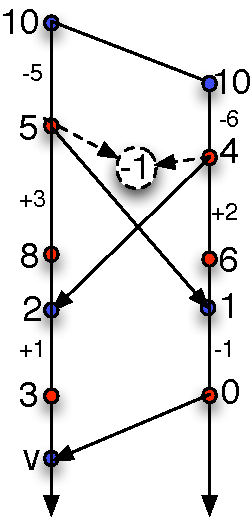
\includegraphics[scale=0.55]{Figures/2-LCAs}
}
\hfill
\subcaptionbox[] {\small
  In this example, latest versions on $b_1$ and $b_3$, and
  $b_2$ and $b_3$ have two LCAs each, hence are unmergeable.
  \label{fig:external-lcas}
} [0.47\columnwidth] {
  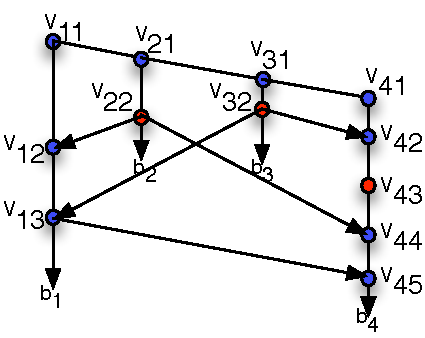
\includegraphics[scale=0.7]{Figures/2-external-LCAs}
}
\caption{Examples where two branches have more than one LCA, hence
cannot merge. }
\label{fig:many-lcas}
\end{figure}

The problem of multiple LCAs also arises in the context of source
control systems, which employ \emph{ad hoc} mechanisms to pave the way
for three-way merging.  Git~\cite{git}, for instance,
recursively merges LCAs by default to compute a virtual ancestor, which then
serves as the LCA for merging concurrent versions. This method is
demonstrated in the branching structure for a mergeable, replicated
counter as shown in Fig.~\ref{fig:criss-cross-lcas}, where LCAs 5 and
4 of 0 and 3 are merged (with their LCA being 10) to generate -1 as
the virtual LCA to merge 5 and 4. A major downside with this approach
is that it makes no guarantees on the relationship between the virtual
ancestor and its concurrent versions; the former may not even be a
legal ancestor of the latter as per the semantics of the data type.
For instance, suppose the integer type in
Fig.~\ref{fig:criss-cross-lcas} represents a bank account balance,
which is expected to disallow any activity on the account if the
balance is ever known to be less than zero.  From the perspective of
the library designer and its clients, there is no meaningful scenario
in which versions 3 and 0 can emerge from -1, since the only
transition allowed by the semantics from -1 is to itself.  Clearly,
\emph{ad hoc} mechanisms like this are error-prone and difficult to
apply in general.

Fortunately, unlike source control systems where branching structure
is entirely dictated by the user, \name abstracts away branching
structure from the programmer, and hence retains the ability to
manifest it in a way that it deems fit. In particular, \name solves
the problem of multiple LCAs by suitably constraining the branching
structure such that the problem never arises. The constraints are
imposed either implicitly, as a result of how the operational semantics
defines an atomic step, or explicitly, by insisting that certain
conditions be met before merging a pair of versions
(\rulelabel{E-Pull-Wait}). First, the operational semantics already
disables criss-cross merges since it only ever merges versions that
are latest on their respective branches. Second, we impose certain
pre-conditions on the merging branches to preempt the structure shown
in Fig.~\ref{fig:external-lcas}. The intuition is as follows: consider
the branch $b_3$ at the instance of merging $v_{12}$. Since it has
already merged $v_{22}$, $v_{22}$ could be a common ancestor for $b_3$
and some other branch (call it $b$). Now, if $b_3$ merges $v_{12}$,
the same could be true of $v_{12}$. Since $v_{12}$ and $v_{22}$ are not
ordered by the ancestor relation, both become LCAs of
$b_3$ and $b$. We observe that this scenario can be prevented if, when
merging $b_1$, $b_3$ insists on an ancestor relation between the last
merged version ($v_{22}$) and the currently merging version.  We call
the last merged version of a branch its \emph{locus}. By maintaining a
total order of among locii of a branch $b$ as new versions are
created, we effectively guarantee the presence of a version (the
locus) that is lower than all the ancestors of the latest version on
$b$. Next, by requiring the locus to be an ancestor of the merging
version, we ensure that all the common ancestors have a single lowest
element, thus enforcing the uniqueness of the LCA.

We now formalize the intuitions described above via a series of
definitions that help us state the guarantees offered by the system.

\begin{definition} [\bfseries Internal and External Ancestors]
Given a branch $b$ and a version $v\in b$, an internal ancestor
($\preceq_i$) of $v$ is an ancestor from the same branch $b$. An
external ancestor ($\preceq_o$) of $v$ is an ancestor from a different
branch $b'\neq b$.
\end{definition}

\begin{definition} [\bfseries Locus]
Given a branch $b$ and a version $v\in b$, the locus ($v_o$) of $v$ is an
ancestor that is not an ancestor of any other external ancestor of
$v$. That is, $\under{H}{v_o \preceq v}$, and there does not exist a
$v_o' \not\in b$ such that $\under{H}{v_o' \preceq v}$ and
$\under{H}{v_o \preceq v_o'}$. We lift the notion of locus to the
level of branches by defining the locus of a branch as the locus of
its latest version.
\end{definition}

\begin{wrapfigure}{l}{.4\textwidth}
\centering
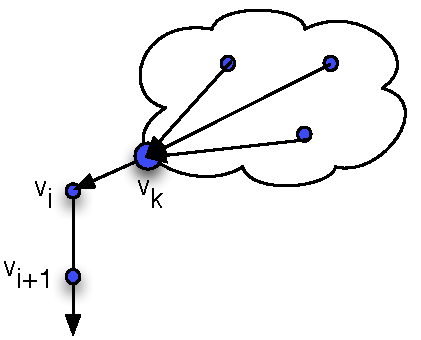
\includegraphics[scale=0.6]{Figures/causal-history}
\caption{The cloud represents the set of all ancestors of versions $v_i$ and
$v_{i+1}$, i.e., their causal history. The locus $v_k$ of both is the
version that succeeds every other ancestor in the causal history.}
\label{fig:causal-history}
\end{wrapfigure}
In a legal branching history, every version has a unique locus
(property follows from Def.~\ref{def:mergeability} below). We define
the \emph{causal history} of a version as the set of all ancestors of
that version. A locus ($v_o$) of a version ($v$) is therefore the
maximum element (lowest element in the ancestor relation) of the
causal history of $v$'s internal ancestor that was the result of the
last merge. This is illustrated in Fig.~\ref{fig:causal-history}. We
make use of this observation while defining mergeability.

\begin{definition} [\bfseries Mergeability]
\label{def:mergeability}
Given a history $H$, a version $v_1$ and a version $v_2$ that is not
an ancestor of $v_1$ under $H$, $v_2$ is mergeable into $v_1$ (denoted
$\under{H}{v_2 \mbleto v_1}$) if and only if the locus ($v_o$) of
$v_1$ is an ancestor of $v_2$, and no internal ancestor of $v_1$ that
is not also an ancestor of $v_o$ is an ancestor of $v_2$.
\end{definition}

If $v_1$ and $v_2$ referred in the above definition are the latest
versions on their respective branches $b_1$ and $b_2$, we say $b_2$ is
mergeable into $b_1$, or more generally, $b_1$ and $b_2$ are
mergeable. The definition essentially requires all of $v_1$'s causal
history that precedes its locus $v_o$ to be included in $v_2$'s causal
history, and none of $v_1$'s history that succeeds $v_o$ to be
included in $v_2$'s history. This allows us to view versions $v_1$ and
$v_2$ as having been independently evolved from a common causal
history whose maximum (w.r.t the ancestor relation) is the version
$v_o$. Consequently, $v_o$ becomes the LCA for $v_2$'s merge into
$v_1$. Generalizing this observation for the latest versions on
any two branches, we state the following theorem:

\begin{theorem} [\bfseries Unique LCA]
Every pair of branches in a legal history $H$, if mergeable as per
Def.~\ref{def:mergeability}, have a unique lowest common ancestor.
\end{theorem}

While the definition of mergeability is sufficient to enforce
uniqueness of LCAs, it may hinder progress in the sense that there may
not exist a pair of branches in a legal history satisfying the
definition, thus making the progress impossible. The following theorem
asserts that this is not the case:

\begin{theorem} [\bfseries Progress]
In a legal branching history $H$ produced by the operational
semantics, if two branches, $b_i$ and $b_j$ are not mergeable (as per
Def.~\ref{def:mergeability}), then there exists a sequence of fork and
merge operations (between mergeable versions) that can be performed on
$H$ to yield a new history $H'$, where $b_i$ and $b_j$ are mergeable.
\end{theorem}

The proof is by the induction on the size of branching history. The
key observation is that the smallest history that is the union of
causal histories of two unmergeable versions (call them $v_i$ and
$v_j$) is smaller than the history that includes the unmergeable
versions. Since causal histories have maximum versions (respective
locii), which, by the inductive hypothesis, can be made mergeable, we
merge them to yield a new version $v$ that is the maximum of the
causal histories of both $v_i$ and $v_j$. If $v_i$ and $v_j$ are the
latest versions on their respective branches, the branches are now
mergeable.

% Observe that $v$ and $v_i$ are mergeable (with
% $v_i$'s locus as the LCA), and so do $v$ and $v_j$. If $v_i$ and $v_j$
% are the latest versions on their respective branches, then merging $v$
% into $v_i$ and $v$ into $v_j$ makes $v$ the locus of both the
% branches, thus making them mergeable again.

% \begin{theorem} [\bfseries Progress and Eventual Convergence] Given a
% legal branching history $H$, and a program $p$, where every thread
% expression in $p$ is a \C{pull}, there exist a series of reduction steps
% that reduce $p; H$ to $p'; H'$, where every thread expression in $p$
% is the same value $v$.
% \end{theorem}
